\documentclass[10pt,journal,a4paper]{IEEEtran}
\usepackage{tikz}
\usepackage{amsmath}
\usepackage{amssymb}
\begin{document}
%
% paper title
% can use linebreaks \\ within to get better formatting as desired
\title{Report for the NOOC project}
\author{Ismail Bouanani and Jean-Baptiste Cordonnier}

\IEEEcompsoctitleabstractindextext{
\begin{abstract}
Rumor spreading is a well known problem with multiple applications, from information broadcast in complex distributed systems to analysis of viral content on social networks. This project report will go over the paper of Guo and Sun \cite{GuoSun}. We aim at providing a good understanding of the concept and the mathematical tool used to show the $O(\log n)$ bound for the time steps needed to spread a rumor. We will then provide simulation of this algorithm on specific graphs.
\end{abstract}
}

\newcommand{\norm}[1]{\left\lVert#1\right\rVert}
\newtheorem{theorem}{Theorem}

% make the title area
\maketitle
\IEEEdisplaynotcompsoctitleabstractindextext

\section{Introduction}

\begin{theorem}[Main result]
  Let $G$ be a graph with $n$ nodes, spectral gap $\alpha$ and irregularity $\beta$. Then there is an explicit protocol using $O(C' \log n) + \tilde O(\log n)$ random bits sucht that with high probability all nodes get the rumor in $T=O(C \log n)$ rounds, where $C = (1/\alpha) \cdot \beta^2 \max(1, 1/(\alpha \cdot \Delta ^ {0.499}))$
\end{theorem}

\section{Rumor spreading protocol}

The rumor spreading protocol is the simplest algorithm we can come with in order to solve the rumor spreading problem. Given a starting node $n_0$ (the source of the gossip), we keep track of a set of informed nodes $S = \{n_0\}$. At each time step of the algorithm, each informed node will select randomly (uniformly to simplify) one of his neighbor and inform him. Step after step the informed nodes set will grow until it contains all the vertex of $G$. Once a node is informed he becomes an informer and will spread the gossip at all the following time steps.

\section{Markov chains set-up}

The analysis in the paper of Guo and Sun \cite{GuoSun} compares the problem of gossip spreading to many random walks in parallel. Whenever a node $u$ pushes the information to an uninformed node $v$, one random walk stays in $u$ and another one goes to $v$. The random walk that "stays" in the same node is called $lazy$ while the other one is non-lazy (or $\overline{lazy}$). This split of random walks represents the fact that the information is now in $u$ and in $v$, $u$ will continue to spread this knowledge in the following rounds.

\begin{figure}[h]
\centering
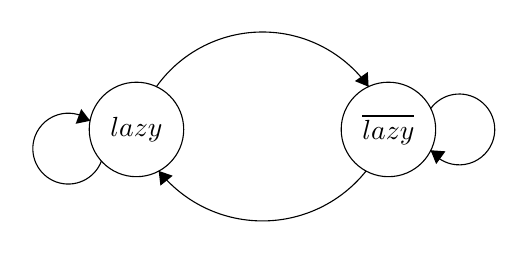
\begin{tikzpicture}[scale=0.2]
\tikzstyle{every node}+=[inner sep=0pt]
\draw [black] (26.1,-26.6) circle (3);
\draw (26.1,-26.6) node {$lazy$};
\draw [black] (42.1,-26.6) circle (3);
\draw (42.1,-26.6) node {$\overline{lazy}$};
\draw [black] (40.688,-29.229) arc (-38.4609:-141.5391:8.413);
\fill [black] (27.51,-29.23) -- (27.62,-30.17) -- (28.4,-29.54);
\draw [black] (27.358,-23.895) arc (144.65362:35.34638:8.265);
\fill [black] (40.84,-23.89) -- (40.79,-22.95) -- (39.97,-23.53);
\draw [black] (23.878,-28.598) arc (-20.31276:-308.31276:2.25);
\fill [black] (23.16,-26.05) -- (22.59,-25.3) -- (22.24,-26.24);
\draw [black] (44.78,-25.277) arc (144:-144:2.25);
\fill [black] (44.78,-27.92) -- (45.13,-28.8) -- (45.72,-27.99);
\end{tikzpicture}
\caption{Random walk state}
\label{fig:lazyFSM}
\end{figure}

We define two types of random walks when the information is spread through the graph: the forward and the backward random walks. Forward random walks start from the source $s$ while backward random walks are used only in the analysis and start from a targeted node $t$. In fact if a node $u$ pushes information to a node $v$, we can also say that $v$ "pulls" the information from $u$ and there exists a random walk called reverse having a step from $v$ to $u$, that remains true if and only if $u$ the only node that pushed to $v$ is $u$.Then to know if a node $t$ has been informed, we only need to show that there exists a node $v$ reached by a forward random walk from $s$ and by a backward random walk from $t$.

We can consider all the random walks pattern after $k$ steps as $S \in \mathcal C_k = \{ lazy, \overline{lazy} \}^k$. We define the indicator random variable $X_{u,v}^S$ (resp. $Y_{u,v}^S$) that the forward (resp. backward) random walk with pattern $S$ and initial node $u$ will end up at node $v$. To show that a node $w$ is reached by the gossip in $T$ step we need to find a vertex $u$ such that $X_{s,u}^{S}Y_{w,u}^{S'} = 1$ with $|S| = |S'| = T/2$.

\section{Bound analysis}

The aim of this lemma is to show that after $k$ rounds, and independently of the pattern followed (we consider the lazy version of the matrix here), any distribution is identical to the stationary distribution $\pi \otimes \pi$ (i.e $P(u,v)=(1/n)^2$) for all $(u,v) \in V[G] \times V[G]$. To do so, we lower bound the quadratic distance

\[
  \norm{u(\mathcal L_{\gamma,\gamma} \circ \mathcal Q(M))^k - \pi \otimes \pi}_2 \leq (1 - \gamma \alpha / 2)^k + 2 \sqrt 2 \gamma \alpha^{-1} n^{-3/2}
\]

The conclusion for that is, the convergence of the process does not depend on the node who has the information first since after $k$ rounds ($k$ big enough), the parallel $2^k$ Markov chains have joint evolutions (or almost).

The intuition behind any case of rumor spreading is that the topology of the graph has a great impact on the efficiency of our algorithm. For instance, nodes very poorly connected and far from the majority of the other nodes will be hard to reach or terrible gossip starter. This essence of "good" and "bad" graphs is captured by the spectral gap $\alpha$ and the irregularity $\beta$. The spectral gap $\alpha$ is defined by $\alpha \triangleq 1 - \lambda_2$ where $\lambda_2$ is the second eigenvalue of the Laplacian matrix associated to the graph. 
Intuition tells us that if there are a lot of edges and no bottlenecks then the flow should spread out quickly and the Markov chain mix rapidly. The irregularity $\beta$ is defined as $\beta \triangleq \Delta/\delta$.

\section{Randomness needed}

\bibliography{biblio.bib}

\end{document}


